%!TEX root = JakubJedryszek-MasterThesis.tex

\cleardoublepage


\chapter{PCA pump prototype implementation and code generation}
\label{pcapumpimpl}

This chapter describes running SPARK Ada programs on BeagleBoard-xM platform (\ref{pcapump:beagleboard}), implementation details of PCA pump prototype (\ref{pcapumpimpl:manual})), code generation from simplified AADL/BLESS models of PCA pump (\ref{pcapumpimpl:codegen}) and overview of not generated parts, which has to be implemented by developer (\ref{pcapumpimpl:codegenimpl}).


\section{Running SPARK Ada programs on BeagleBoard-xM}
\label{pcapumpimpl:beagleboard}

To run SPARK Ada program on BeagleBoard-xM, it has to be cross-compiled. As an IDE for SPARK Ada development, GNAT Programming Studio (GPS) is used (see section \ref{background:spark:gps}). To create "Hello, World!" application, new Ada project has been created (choosing Project/New... from the menu). Then main.adb file with procedure Main printing "Hello, World!" in standard output was added. The code is presented in listing \ref{listing:HelloWorld}. It is valid Ada 2005 and Ada 2012 code.

\begin{lstlisting}[language=ada, frame=single, gobble=0, caption={"Hello World" in Ada}, label={listing:HelloWorld}]
with Ada.Text_IO;

procedure Main
is
begin
    Ada.Text_IO.Put_Line("Hello, World!");    
end Main;
\end{lstlisting} 

To run it locally, the main file has to be added to the list of 'main files' in Project/Edit Project Properties (figure \ref{figure:editprojectproperties}), tab: Main files (figure \ref{figure:mainfiles}). Then it can be run in GPS, using 'Build All' and 'Run Main' by clicking appropriate toolbar buttons. The main file has to be always specified in order to compile and link application, which is runnable.

\begin{figure}[ht]%t=top, b=bottom, h=here
    \begin{center}
    	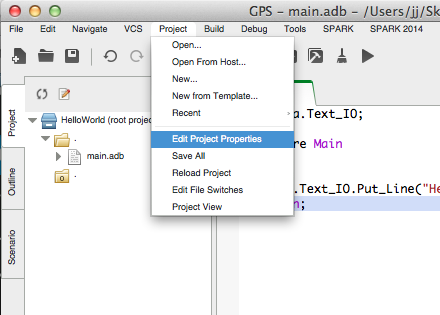
\includegraphics[width=3.2in]{figures/EditProjectProperties.png}
    	\caption{Edit Project Properties}
    \end{center}
    \label{figure:editprojectproperties}
\end{figure}

\begin{figure}[ht]%t=top, b=bottom, h=here
    \begin{center}
    	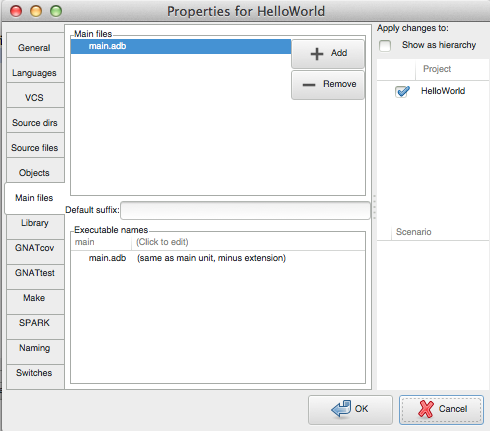
\includegraphics[width=3.2in]{figures/Properties-MainFiles.png}
    	\caption{Project Main files}
    \end{center}
    \label{figure:mainfiles}
\end{figure}

To run it on BeagleBoard-xM we have to use cross-compiler and issue following command: \lstinline{arm-linux-gnueabi-gnatmake -d -Phelloworld.gpr} (helloworld.gpr is GNAT Programming Studio project file). We can specify additional flags in command line or directly in project file (manually or through GNAT Programming Studio Interface).


\subsection{Multitasking applications}
\label{pcapumpimpl:beagleboard:multitasking}

In Ada World, concurrency is referred as tasking and the task is the same construct as the thread in other programming languages. 


\subsection{Controlling PCA pump motor}
\label{pcapumpimpl:beagleboard:pcapumpmotor}





\section{Implementation based on Requirements Document and AADL models}
\label{pcapumpimpl:manual}

In this thesis, only the operation module is implemented. Req doc don't specified all implementation details, like how basal rate should be infused.

The first step, was to check if implementation of PCA Pump specified in Requirements Document is possible. Especially whether it will work on BeagleBoard-xM device. To do that, simple version of PCA Pump based on Requirements Document was created. Only two AADL threads are implemented: \lstinline{Rate_Controler} and \lstinline{Max_Drug_Per_Hour_Watcher} in stripped version.

Pump internal implementation based on \cite{CADD-PrizmAmbulatoryInfusionPump:Online}.
- basal dose deliver in increments - easier to track delivered amount (page 14)

The pump has three tasks in total:
\begin{itemize}
    \item main task (requesting boluses, displaying volume infused etc.)
    \item rate controller - to control the speed of infusion rate
    \item max drug per hour watcher - to control overinfusion
\end{itemize}

The main PCA Pump Package can be verified using SPARK tools. The Pump engine (motor) is separated entity. It has an interface allowing request infusion of 0.1 ml of drug.

PCA Pump prototype was developed based on Requirements Documentation created by Brian Larson, John Hatcliff and Partice Chalin \cite{PcaReq}.


\section{Code generation from AADL/BLESS models}
\label{pcapumpimpl:codegen}

PCA Pump prototype was mocked using translations schemas from chapter \ref{codegen}.

The original models were simplified and truncated for the purpose of this thesis. Finally only \lstinline{PCA_Operation} module with 3 threads (\lstinline{Max_Drug_Per_Hour_Watcher}, \lstinline{Rate_Controller}, \lstinline{Patient_Bolus_Checker}), types definitions (\lstinline{Base_Types}, \lstinline{PCA_Types}, \lstinline{ICE_Types}, \lstinline{Bless_Types}) and property set \lstinline{PCA_Properties} were used as the source for code translation.

[code listings of aadl model]


Skeleton code 'generated' from simplified AADL models. Then implemented.

Show generated code.



\section{Implementation for generated code}
\label{pcapumpimpl:codegenimpl}

Mocked code was extended (e.g. to Prescription\_Store Set/Get methods for record fields were added).

Overview of issues solved: 
* Bolus options: FBasal + FPatient or FPatient => implemented: FBasal + FPatient (consistent in doc)
5 modes:
* Stopped: F=0
* KVO: F=0.1
* Basal: F=Fbasal
* Patient: F = Fbasal + Fbolus (for vtbi/Fbolus)
* Clinician: F = Fbalsal + Fbolus (for specified time)

Most common Examiner\cite{Examiner:Online} erroes/warnings:
***        Warning                     :302: This expression may be
***        Semantic Error              :725: Protected function or variable XXX may only appear directly in an assignment or return statement.

Discuss implementation of basal infusion: 0.1 ml pulses timed according to the desired rate. (based on CADD-Prizm page 14). Easier bolus monitoring/calculations. Possibility to separate pulse from engine logic. Just array with time stamps(?) or array with size = (60 * 60 /min\_possible\_time\_between\_activations) and set 1 if activation occured. In every second, update array: array[i]=array[i+1]. Array is protected object, so bolus thread cannot access it in the same time, when update thread.
Another option: constant speed of engine and speed-up on boluses. Harder bolus monitoring/calculations?


Internal calculations are in micro liters 1 micro liters ($\mu$l) = 0.001 ml thus 1 ml = 1000$\mu$l.


